% Chapter 2

\chapter{The Existing Annotator System} % Main chapter title

\label{Chapter2} % For referencing the chapter elsewhere, use \ref{Chapter1} 

\lhead{Chapter 2. \emph{The Existing Annotator System}} % This is for the header on each page - perhaps a shortened title

%----------------------------------------------------------------------------------------

\section{Overview of Annotator}
The beta version of Siyavula's Annotator software allowed people to highlight HTML text in a webbook and make an annotated comment about their selection. In order to use the annotator, users had to be be logged in so that their annotations could be correctly attributed to them. 

\begin{figure}[h]
    \centering
    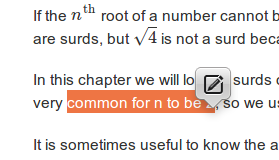
\includegraphics[width=0.4\textwidth]{Figures/annotator1.png}
 \caption{Highlighted text with the ``Annotate'' icon}
\end{figure}

Annotations could be made in one of three categories: errata, suggestion and comment.
\begin{figure}[h]
    \centering
    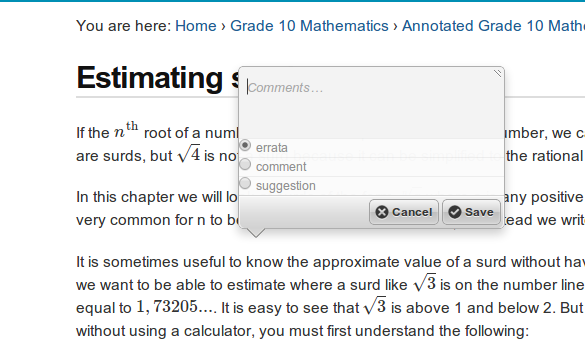
\includegraphics[width=\textwidth]{Figures/annotatorcategories.png}
 \caption{Three categories of annotation}
\end{figure}

They were then stored in a database for future reference. All users could view existing annotations on a webpage when they logged in to the annotated version of the webbook. Users could also reply to existing annotations made by themselves, or other users.

%-----------------------------------------
\section{Technical details of Annotator}
The annotation software Siyavula decided to utilise (and modify for the company's own purposes) is based on an open source application called ``Annotator"\footnote{\href{ http://okfnlabs.org/annotator/}{ http://okfnlabs.org/annotator/}} (forked by Siyavula's developer at \href{https://github.com/ezietsman/annotator}{https://github.com/ezietsman/annotator}). Annotator is a Javascript application that is written in Coffeescript. It uses a Couch database and has a Python server back-end. It does not come packaged with any functional user interface for the viewing of saved annotations outside of the webpage where they were made.

Siyavula's version of Annotator ran on static versions of the company's webbooks, not on the latest live versions.

%-----------------------------------------
\section{Existing Interface}
The backend interface for the annotator consisted of a simple table list of annotations.

Table columns included: ``Type", ``id" (the database primary key), ``Comment" (the text typed by the user), ``User", ``Time" (date and time) and ``URL" (the webpage on which the annotation was made.) Most recent annotations were listed first. The type of annotation was also indicated by one of three colours in the left hand column.
\begin{figure}[h]
    \centering
    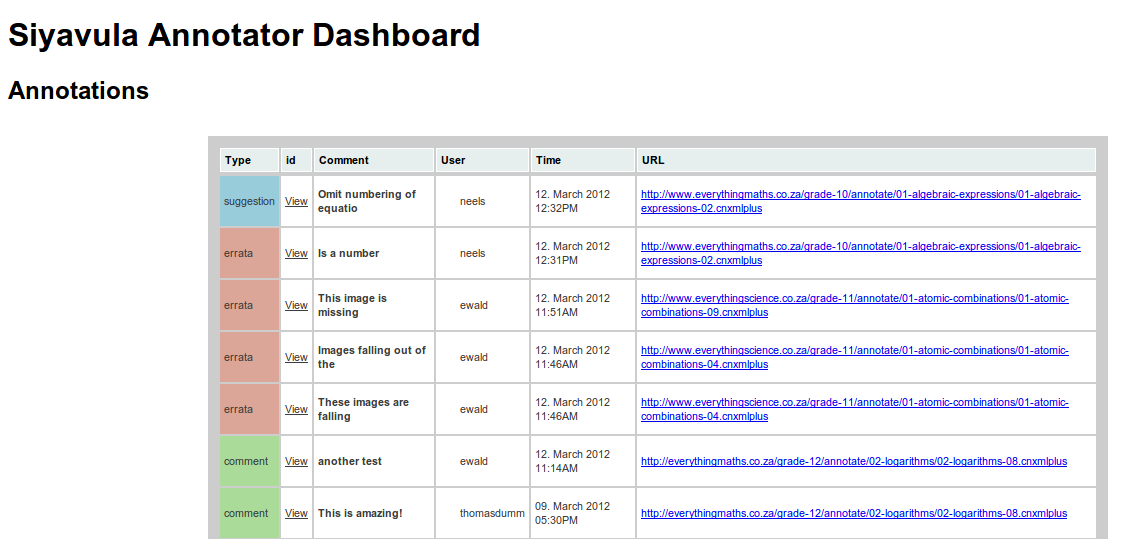
\includegraphics[width=\textwidth]{Figures/annotator-backend-table.png}
 \caption{The existing back-end interface: a simple table of stored annotation data}
\end{figure}

Columns were not sortable, and there was no search or filter mechanism. The back-end merely provided a list of annotations, with some basic information about each entry. For in-house processing of small numbers of annotations ( $<$ 20), this basic back-end was adequate (albeit  very rough) for advanced members of the team. However, this interface was not scalable (processing $>$ 100 annotations listed like this would be extremely difficult) and not user-friendly at all, particularly for less technologically advanced employees. Indeed, it had not been designed with any user requirements in mind at all - it had merely been cobbled together as a temporary way to view annotations that had been made.

Given the simplicity of the existing interface and the potential for a functional annotator to be an integral part of many stages of Siyavula's book-writing and -maintaining process, it was decided that there would be immense value in designing a unique back-end interface. This interface could be tailored to accommodate different team members' specific user requirements and therefore help to maximise the use of the annotator as a functional tool for making, storing, processing and resolving annotations containing volunteer and general feedback.
